\documentclass[a4paper]{jpconf}
\usepackage{graphicx}
\usepackage[margin=0.8in]{geometry}
\usepackage{lmodern}% http://ctan.org/pkg/lm
\usepackage{listings}
\usepackage[utf8]{inputenc}
\usepackage[toc,page]{appendix}
%\usepackage{wrapfig}
%\usepackage{float}
\usepackage{hyperref}
\usepackage{listings}
\usepackage{citesort}
\usepackage{changepage}
\usepackage{caption}
\usepackage{color}
\usepackage{courier}
\usepackage{subcaption}
\usepackage{hyperref}\begin{document}
\title{Profiling ATLAS Kit Validation on \newline Intel Haswell-EP processors}

\author{M Guerri$^1$, D Giordano$^1$, C Cordeiro$^1$}
\address{$^1$ CERN}
\ead{marco.guerri@cern.ch}

\definecolor{lightblue}{gray}{0.95}

\lstset{
    language=Python,
    basicstyle=\sffamily,
    tabsize=2,
    backgroundcolor=\color{lightblue},
    captionpos=b,
    %numbers=left,
    columns=1,
    keepspaces=true,
    showstringspaces=false,
    stepnumber=1,
    numberstyle=\scriptsize,
    numbersep=5pt,
    frame=lines,
    escapeinside={£}{£},
    breaklines=true,
    keywordstyle=\color[rgb]{0,0,1},
    commentstyle=\color[rgb]{0.133,0.545,0.133},
    stringstyle=\color[rgb]{1,0,0}
}

\input{Intro}

%\section{Bare metal results}
In order to ease the performance analysis, the virtualisation layer was
temporarily removed and Simultaneous Multithreading disabled, running KV on 
the bare-metal server while setting scheduling affinity sequentially to each physical
core. The results shown
in Figure~\ref{kv-runtime} highlighted a 12\% difference in the average simulation
time when binding KV to core 8, the first core of the second processor, i.e. CPU1.

\begin{figure}[b]
\begin{center}
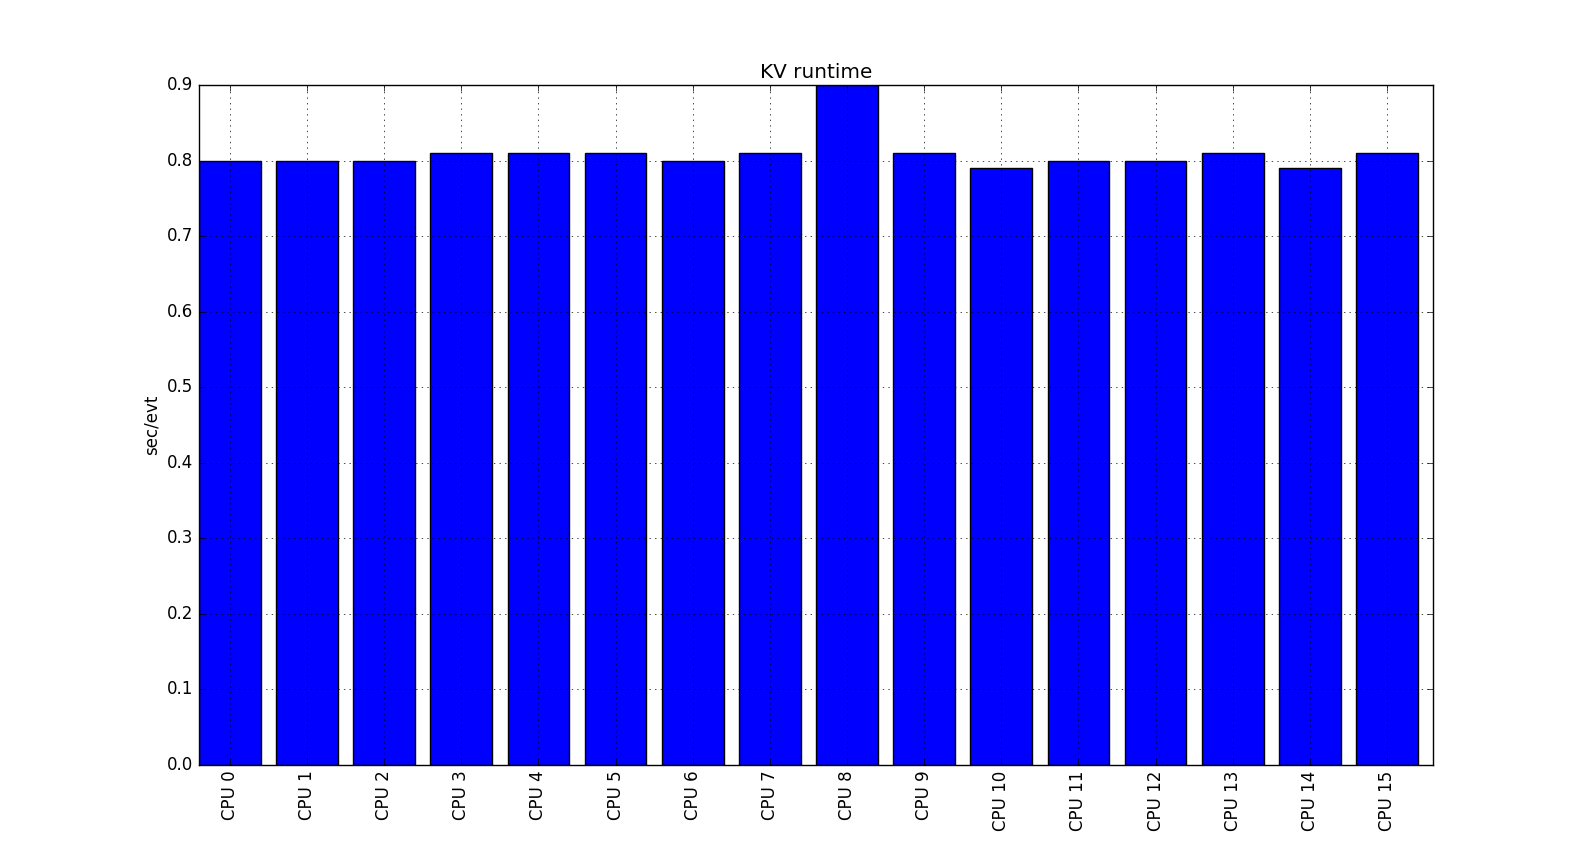
\includegraphics[scale=0.3]{images/kv_runtime.png}
\end{center}
\caption{\label{kv-runtime} Bare-metal KV performance (sec/evt) on each physical core. }
\end{figure}
Further tests confirmed the same behaviour also with Simultaneous Multithreading 
on, with slower performance on thread 8 and 24, both belonging to the first core of 
CPU1. Single thread runs in a virtualised environment showed a 16\%
increase in the final average simulation time when running on virtual processors
corresponding to hardware threads 8 and 24, confirming the 2\%
spread that stood out from the statistical distribution after averaging the results
over all 8 virtual processors within each VM. 


\section{Profiling single events}
A deeper dive in the logs showed that all the events required more time to be 
simulated on the first core of CPU1. In particular, event 73 was identified as the one
requiring the longest simulation time: ~34 seconds on core 8 against ~29 seconds
on any other core, making it a good candidate for an in-depth analysis. Profiling 
a single event required a way to attach \textit{perf} to KV only during the time frame
where one specific simulation was being executed. The solution adopted consisted
in a Python script which would monitor KV log files via \textit{pyinotify} to detect
the beginning of event 73. The script would attach \textit{perf} to KV until the
detection of the end of event. One essential requirement for this to work correctly
was to disable all the buffering carried out at any layer of the stack before
data actually reaching the storage device. KV writes log files via Python code,
therefore the following points had be taken into consideration:
%\begin{lstlisting}[caption=Simulation of event 73 on core 8, basicstyle=\scriptsize]
%*  Memory snooper called at end of event with VMEM: 1443232kB
%G4SimTimer           INFO        Event nr. 73 took 34.58 s. New average 0.985 +- 0.4806
%AtRndmGenSvc         INFO  Stream =  SINGLE, Seed1 =  93448506, Seed2 = 144728191
%AthenaEventLoopMgr   INFO  done processing event #72, run #1 73 events processed so far
%AthenaEventLoopMgr   INFO  start processing event #73, run #1 73 events processed so far
%G4AtlasAlg           INFO ++++++++++++  G4AtlasAlg execute  ++++++++++++
%\end{lstlisting}

%\begin{lstlisting}[caption=Simulation of event 73 on core 0, basicstyle=\scriptsize]
%*  Memory snooper called at end of event with VMEM: 1443252kB
%G4SimTimer           INFO        Event nr. 73 took 29.68 s. New average 0.8681 +- 0.4133
%AtRndmGenSvc         INFO  Stream =  SINGLE, Seed1 =  93448506, Seed2 = 144728191
%AthenaEventLoopMgr   INFO  done processing event #72, run #1 73 events processed so far 
%AthenaEventLoopMgr   INFO  start processing event #73, run #1 73 events processed so far
%G4AtlasAlg           INFO ++++++++++++  G4AtlasAlg execute  ++++++++++++
%\end{lstlisting}

\begin{itemize}
\item A call to \textit{open} function in Python, results in the invocation
of libc \textit{fopen}. Python can modify libc buffering behaviour via libc 
function \textit{setvbuf} if \textit{buffering} parameter is specified, 
otherwise the default libc buffering is used. Without control over the Python
source code, its it not possible to modify buffering options.
\item Environment variable \textit{PYTHONUNBUFFERED} can be used to turn off
buffering of \textit{stdin, stdout, stderr}.. 
\end{itemize}
The best solution found to implement unbuffered I/O to log files was to set 
\textit{PYTHONUNBUFFERED=1} and pipe logs printed by KV on standard output to
\textit{tee}, which would eventually write to an additional log file setting 
\textit{\_IONBF} on all file descriptors via \textit{setvbuf}.
\textit{unbuffer} command was also used to disable buffering between the two
ends of the pipe. 
\\
\textit{perf record} was used to profile the execution. Results for core 8 
and core 0 are shown respectively in figure ~\ref{event-73-processor8} and 
figure ~\ref{event-73-processor0} (limiting the output to the functions that
account for more than 1\% of the runtime). 

\begin{figure}[h]
\begin{center}
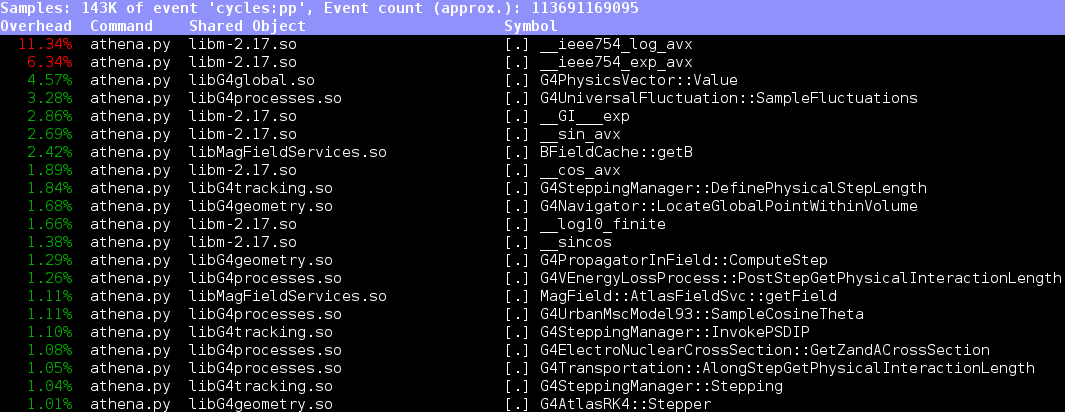
\includegraphics[scale=0.45]{images/Event73_Processor8.png}
\end{center}
\caption{\label{event-73-processor8} Recording of event 73 on core 8}
\end{figure}

\begin{figure}[h]
\begin{center}
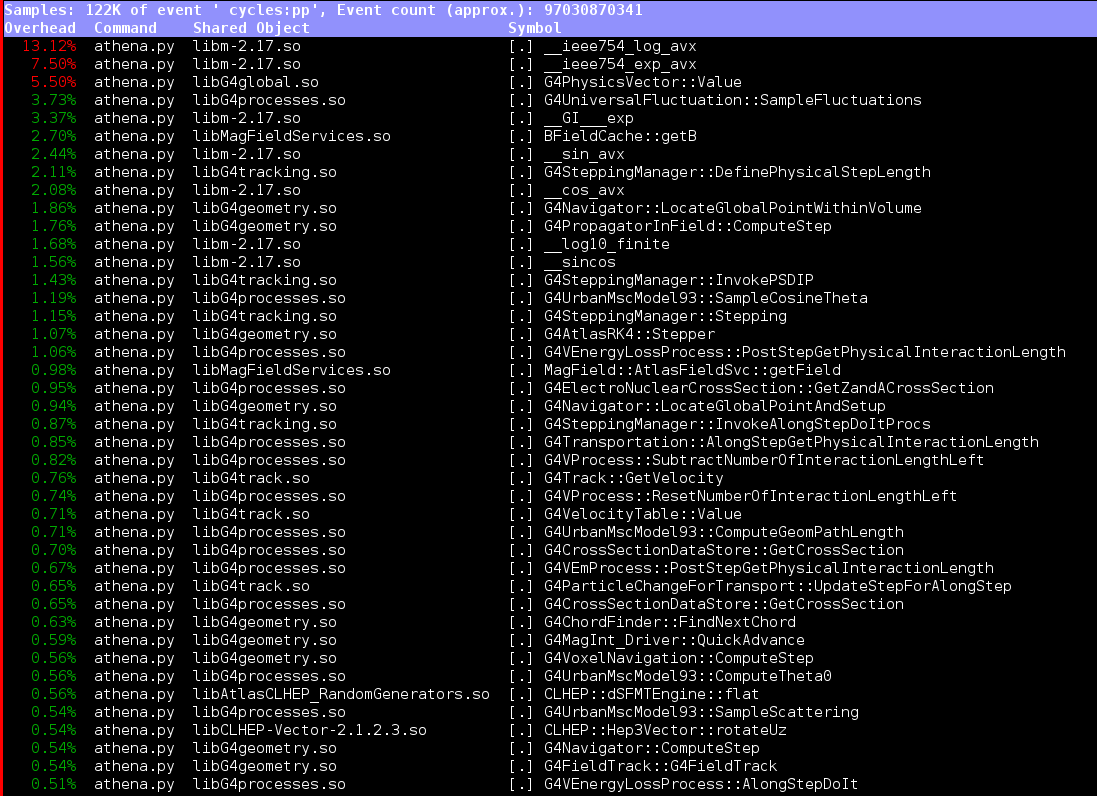
\includegraphics[scale=0.45]{images/Event73_Processor0.png}
\end{center}
\caption{\label{event-73-processor0} Recording of event 73 on core 0}
\end{figure}

Excluding the higher number of events
(unhalted core cycles) on core 8, which was expected due to the longer runtime,
it was not possible to identify any major difference between the two runs, which
were showing the same functions coming mostly from \textit{libm} and \textit{Gean4} 
functions. These results were then elaborated into a list of the top contributors 
to the additional clock cycles required when running on core 8 as shown 
in table ~\ref{major-contributors}.

\begin{table}
\begin{center}
\begin{tabular}{ | l | l |}
    \hline
	\_\_sin\_avx & 4.14\% \\
	\hline
	G4VEnergyLossProcess::PostStepGetPhysicalInteractionLength & 2.40\% \\
    \hline
 	FADS::FadsSteppingAction::UserSteppingAction & 2.26\% \\
    \hline
	G4Transportation::AlongStepGetPhysicalInteractionLength & 2.18\% \\
    \hline
	G4ParticleChangeForTransport::UpdateStepForAlongStep & 2.07\% \\
    \hline
	MagField::AtlasFieldSvc::getField & 1.86\% \\
    \hline
	G4ElectroNuclearCrossSection::GetZandACrossSection	& 1.85\% \\
	\hline
	G4Tubs::DistanceToOut & 1.62\% \\
	\hline
	G4CrossSectionDataStore::GetCrossSection & 1.59\% \\
	\hline
	\_\_log10\_finite &	1.53\% \\
	\hline
\end{tabular}
\end{center}
\caption{Major contributors to the additional runtime on core 8 (percentage
of the additional clock cycles) }
\label{major-contributors}
\end{table}

\section{Profiling the major contributors}
After having obtained the list in table ~\ref{major-contributors}, the 
top contributors to the additional runtime were profiled to obtain
a detailed breakdown of the weight of each assembly instruction in terms of 
clock cycles. The recordings for \textit{\_\_sin\_avx}, 
\textit{PostStepGetPhysicalInteractionLength}, \textit{UserSteppingAction},
\textit{UpdateStepForAlongStep} are reported in Appendix  
~\ref{appending:function-recording}. The results highlighted an interesting 
pattern on most of the major contributors:  it appeared that an unexpectedly 
large number of cycles was attributed to the initial instructions of each function.
Most of these instructions, despite sometimes accessing memory 
(e.g. push on the stack), could not justify such a high cost: in some cases a 
\textit{mov} of a literal value to a register was taking up 8\% of the whole 
execution time of that specific function. Such behavior was common to all cores,
but if these functions were responsible for most of the additional execution time,
then probably the reason had to be related to this peculiar profile. A first hypothesis
pointed in the direction of instruction cache misses as the reason behind
the large number of cycles spent on the initial instructions 
ATLAS Kit Validation seemed a good candidate for a large number of  such events,
with its large code segment consisting of tens of shared libraries. Even though,
this hypothesis could not explain the slower performance when running on core 8,
an attempt was made to validate it.
 

\section{Synthetic benchmark to generate instruction cache miss}
A synthetic benchmark aimed at causing a large number of instruction cache 
misses was generated with the Python script in Appendix 
~\ref{appendix:synthetic-benchmark-cache-misses}. The resulting C code was compiled
under CentOS 7 with gcc 4.8.5 and \textit{-O0}. The benchmark consists of a large
number of dummy functions which are called randomly at runtime, resulting in
repeated instruction cache misses in L1i and L2. Interestingly, the results
highlighted the same performance asymmetry observed with ATLAS Kit Validation.
%as shown in figure ~\ref{syn-bench-a}. 
The runtime on core 8 is 20\% higher in this case.

%\begin{figure}[h]
%\begin{center}
%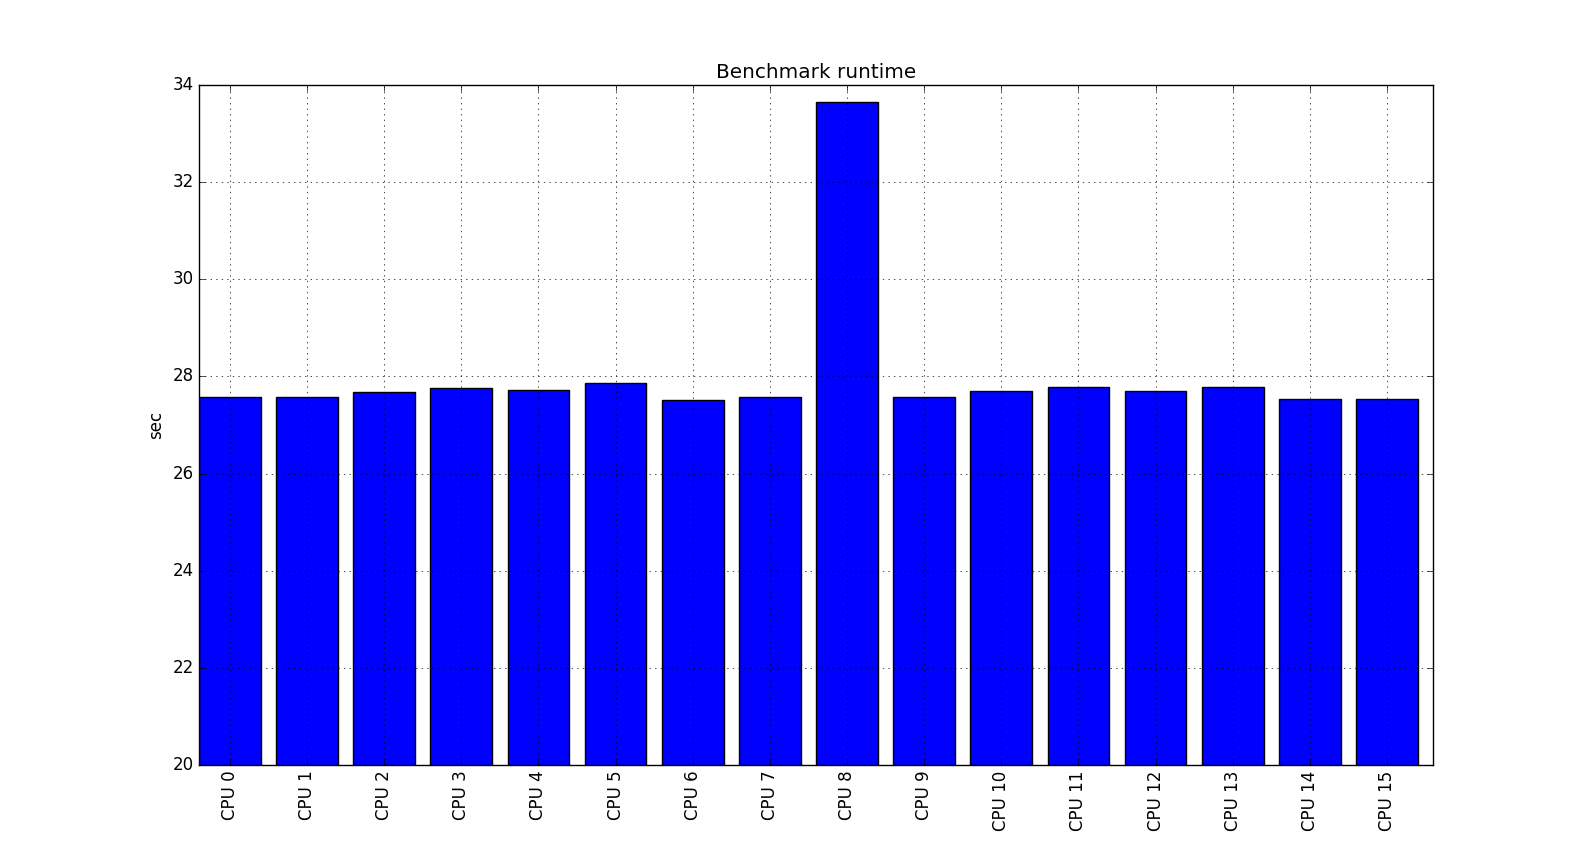
\includegraphics[scale=0.45]{images/syn-bench-a.png}
%\end{center}
%\caption{\label{syn-bench-a} Runtime of the synthetic benchmark (random calls)}
%\end{figure}

However, further investigations succeeded in reproducing 
workloads with similar relative number of L1i and L2 instruction cache misses,
but without any runtime discrepancy, disproving the initial hypothesis.

\section{Additional benchmark with customizable code segment size}
A second synthetic benchmark was written in order to verify the existence of a 
possible correlation between the size of the code segment and the performance 
asymmetry. This benchmark is also aimed at generating instruction cache misses,
but within a code segment whose size can be controlled via a command line 
argument. The code makes use of a large switch statement that dispatches
opcodes randomly generated. This operation is performed in loop: 
by feeding the switch with $opcode \pmod n$, the number of case 
branches effectively used is limited to $n$. The higher $n$, the larger the
number of case branches that can be reached. By ``sampling'' the 
maximum and minimum values of \textit{rip} register, a reliable estimate of the 
size of the hot portion of the code segment is provided. The
benchmark accepts $n$ as command line argument and prints a tuple consisting of
three values: \textit{(size code segment, runtime without initialization, n)}.
The graph in figure shows the difference in runtime between core 8 and core 0
with a code segment of increasing size.














\begin{appendices}

\section{Function recordings}
\label{appending:function-recording}
\begin{figure}[H]
\begin{center}
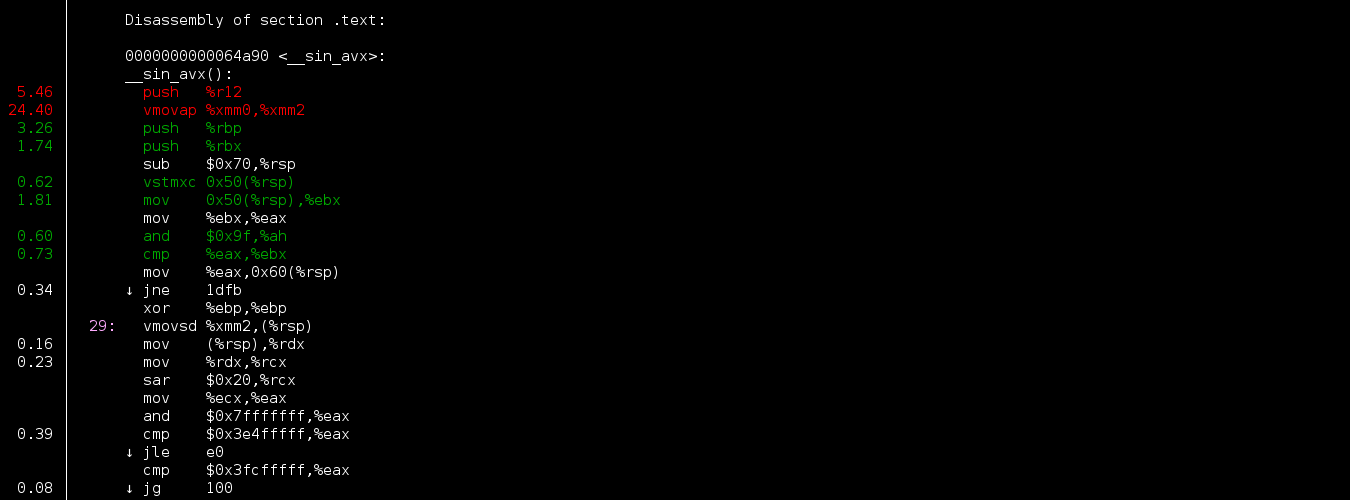
\includegraphics[scale=0.35]{images/sin_P8.png}
\caption{\_\_sin\_avx}
\end{center}
\end{figure}

\begin{figure}[H]
\begin{center}
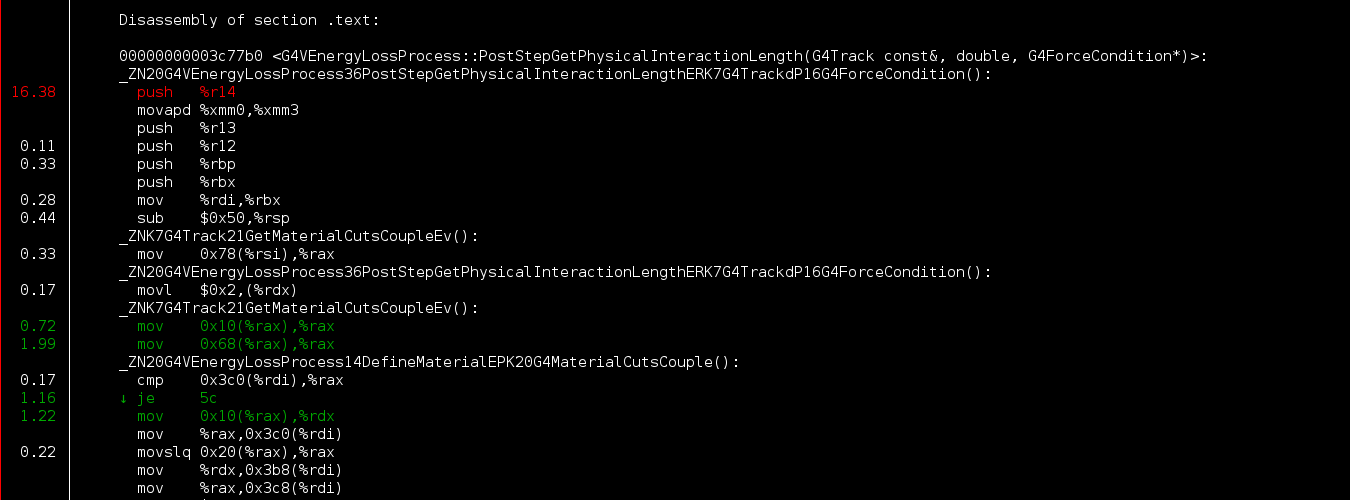
\includegraphics[scale=0.35]{images/Post_step_P8.png}
\caption{PostStepGetPhysicalInteractionLength}
\end{center}
\end{figure}

\begin{figure}[H]
\begin{center}
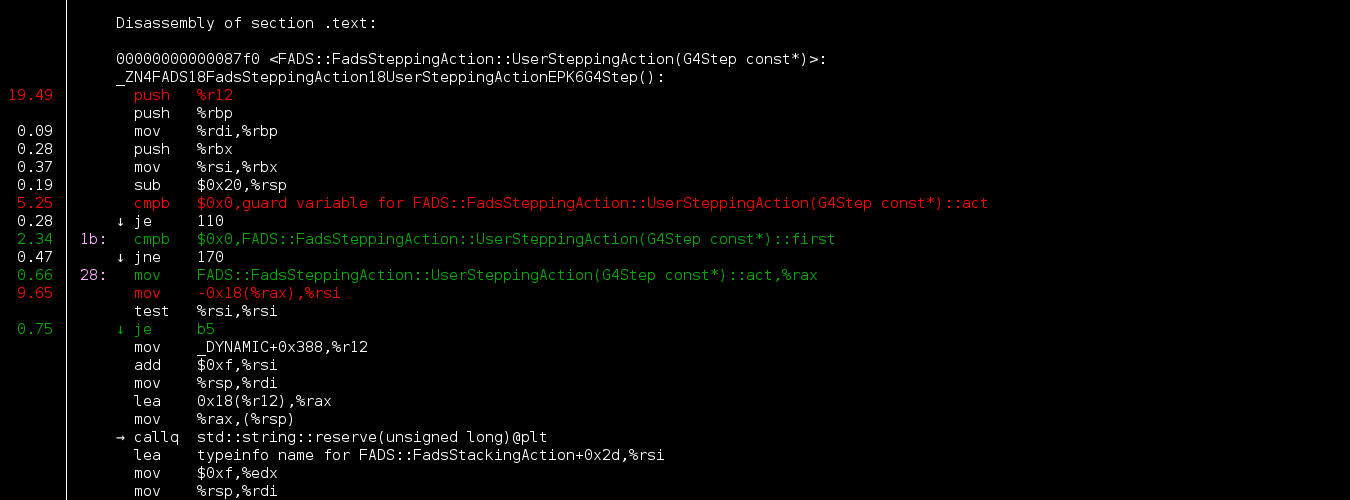
\includegraphics[scale=0.35]{images/UserStepping_P8.png}
\caption{UserSteppingAction}
\end{center}
\end{figure}

\begin{figure}[H]
\begin{center}
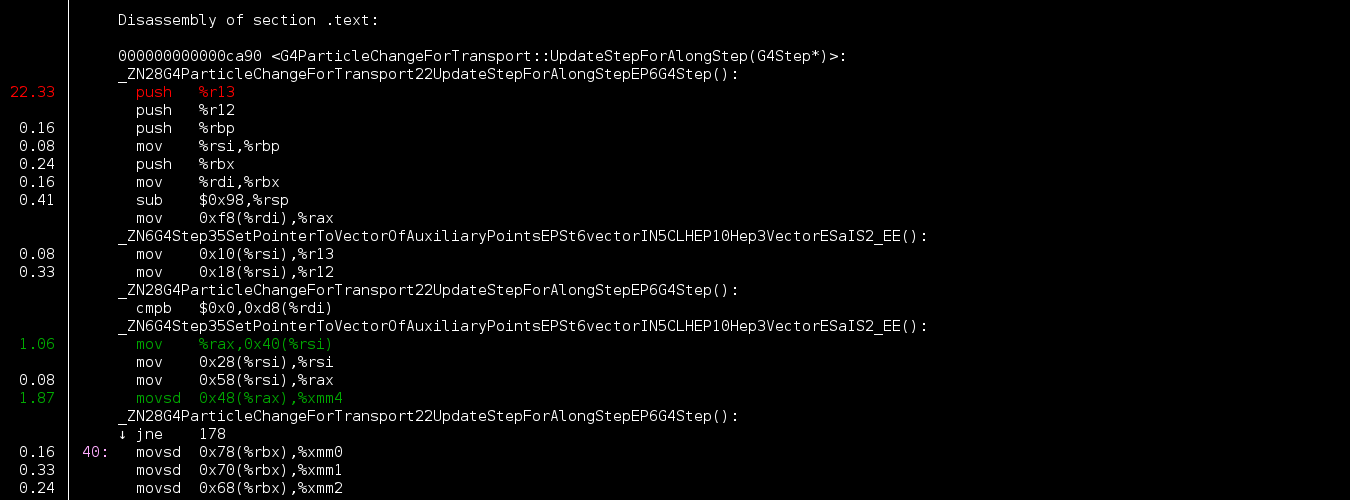
\includegraphics[scale=0.35]{images/UpdateForAlongStep_P8.png}
\caption{UpdateStepForAlongStep}
\end{center}
\end{figure}

\section{Synthetic Benchmark - Cache misses}

\label{appendix:synthetic-benchmark-cache-misses}
\begin{lstlisting}[caption=Python code which generates the synthetic benchmark]]
#!/usr/bin/env python
import tempfile
import random
import sys

if __name__ == '__main__':
    functions = list()
    for i in range(10000):
        func_name = "f_{}".format(next(tempfile._get_candidate_names()))
        sys.stdout.write("void {}() {{\n".format(func_name))
        sys.stdout.write("    double pi = 3.14, r = 50, h = 100, e = 2.7, res;\n")
        sys.stdout.write("    res = pi*r*r*h;\n")
        sys.stdout.write("    res = res/(e*e);\n")
        sys.stdout.write("}\n")
        functions.append(func_name)
    sys.stdout.write("int main() {\n")
    sys.stdout.write("unsigned int i;\n")
    sys.stdout.write("for(i =0 ; i < 100000 ;i ++ ){\n")
    j = 0
    for i in range(10000):
        r = random.randint(0, len(functions)-1)
        sys.stdout.write("{}();\n".format(functions[r]))
    sys.stdout.write("}\n")
    sys.stdout.write("}\n")
\end{lstlisting}

Code listed in Appendix ~\ref{appendix:synthetic-benchmark-cache-misses} can be found 
\href{www.google.it}{online}.

\section{Synthetic Benchmark - iTLB misses}
\label{appendix:synthetic-benchmark-itlb} 
\begin{lstlisting}[caption=Synthetic benchmark using a code segment of adjustable size, language=c]
#include <stdint.h>
#include <stdlib.h>
#include <time.h>
#include <memory.h>
#include <stdlib.h>
#include <stdio.h>
#include <time.h>

uint64_t max_ip = 0, min_ip = 0;
uint64_t ip;

#define RNG_LEN 100000
#define N_ITER 0x2FFFFFFE

#define CASE(N) \
            case N: \
            {       \
                __asm__  volatile("lea 0x0(%%rip), %%rax\n\t"  \
                  "movq %%rax, %0\n\t" \
                  : "=m" (ip)           \
                  : \
                  : "%rax"); \
                max_ip = max_ip ^ ((ip ^ max_ip) & -(ip > max_ip)); \
                break; \
            }
#define CASE2(N) \
            CASE(N) \
            CASE(N+1)

#define CASE4(N) \
            CASE2(N) \
            CASE2(N+2)

#define CASE8(N) \
            CASE4(N) \
            CASE4(N+4)

#define CASE16(N) \
            CASE8(N) \
            CASE8(N+8)

#define CASE32(N) \
            CASE16(N) \
            CASE16(N+16)

#define CASE64(N) \
            CASE32(N) \
            CASE32(N+32)

#define CASE128(N) \
            CASE64(N) \
            CASE64(N+64)

#define CASE256(N) \
            CASE128(N) \
            CASE128(N+128)

#define CASE512(N) \
            CASE256(N) \
            CASE256(N+256)

#define CASE1024(N) \
            CASE512(N) \
            CASE512(N+512)

#define CASE2048(N) \
            CASE1024(N) \
            CASE1024(N+1024)

#define CASE4096(N) \
            CASE2048(N) \
            CASE2048(N+2048)

#define CASE8192(N) \
            CASE4096(N) \
            CASE4096(N+4096)

#define CASE16384(N) \
            CASE8192(N) \
            CASE8192(N+8192)

#define CASE32768(N) \
            CASE16384(N) \
            CASE16384(N+16384)

int main(int argc, char* argv[])
{

    /* boundary is uint32 to support case statements > 65536 */
    uint32_t boundary, *random_sequence, i, opcode;
    struct timespec start, end;

    if(argc < 2) {
        printf("Code segment size must be specified.\n");
        printf("The size of the code segment is roughly switch_size*89\n");
        exit(1);
    }
    boundary = atoi(argv[1]);

    random_sequence = (uint32_t*)malloc(sizeof(uint32_t)*RNG_LEN);
    for(i=0; i< RNG_LEN; i++)
        random_sequence[i] = rand() % boundary;

    clock_gettime(CLOCK_MONOTONIC, &start);
    __asm__  volatile("lea 0x0(%%rip), %%rax\n\t"
          "movq %%rax, %0\n\t"
          : "=m" (ip)
          :
          : "%rax");
    i = 0;
    min_ip = ip;
    while(1) {
        if (i > N_ITER)
           break;
        opcode = random_sequence[i % RNG_LEN];
        switch(opcode)
        {
            CASE32768(0);
        }
    i++;
    }
    clock_gettime(CLOCK_MONOTONIC, &end);
    double time = (end.tv_sec - start.tv_sec) + (end.tv_nsec - start.tv_nsec)/1000000000.0;
    printf("%lu %f %d\n", max_ip - min_ip, time,atoi(argv[1]));
    return 0;
}
\end{lstlisting}

Code listed in Appendix ~\ref{appendix:synthetic-benchmark-itlb} can be found 
\href{www.google.it}{online}.

\end{appendices}
\section*{References}
\bibliography{iopart-num}
\bibliographystyle{unsrt}
\end{document}
